\chapter{Results}
\subsection{Ablation Study on Loss Components}
\label{sec:ablation_loss}

To evaluate the contribution of each loss component to the overall model performance, an ablation study was conducted. 
Four training configurations were compared:
\begin{enumerate}
    \item $\mathcal{L}_{\text{GAN}} + \mathcal{L}_{\text{L1}}$,
    \item $\mathcal{L}_{\text{GAN}} + \mathcal{L}_{\text{L1}} + \mathcal{L}_{\text{SSIM}}$,
    \item $\mathcal{L}_{\text{GAN}} + \mathcal{L}_{\text{L1}} + \mathcal{L}_{\text{LPIPS}}$, and
    \item the full combination $\mathcal{L}_{\text{GAN}} + \mathcal{L}_{\text{L1}} + \mathcal{L}_{\text{SSIM}} + \mathcal{L}_{\text{LPIPS}}$.
\end{enumerate}

This analysis aimed to isolate the effect of each additional loss term on both quantitative metrics and visual reconstruction quality. 
The evaluation was performed using standard image similarity metrics, including Peak Signal-to-Noise Ratio (PSNR), Structural Similarity Index Measure (SSIM), and the Learned Perceptual Image Patch Similarity (LPIPS) score.

\subsubsection*{Quantitative Results}
Table~\ref{tab:ablation_quantitative} summarizes the quantitative performance across the four configurations. 
The results demonstrate the incremental benefit of incorporating perceptual and structural similarity terms alongside the adversarial and $\mathrm{L1}$ objectives.

\begin{table}[h!]
\centering
\caption{Quantitative results of the ablation study across different loss configurations. Arrows ($\uparrow$ / $\downarrow$) indicate whether higher or lower values denote better performance, respectively. 
Best values per metric are shown in bold.}
\label{tab:ablation_quantitative}
\begin{tabular}{lcccccc}
\toprule
\textbf{Loss Configuration} & \textbf{SSIM $\uparrow$} & \textbf{PSNR (dB) $\uparrow$} & \textbf{LPIPS $\downarrow$} & \textbf{SAM~(°) $\downarrow$} & \textbf{MAE $\downarrow$} & \textbf{RMSE $\downarrow$} \\
\midrule
$\mathcal{L}_{\text{GAN}} + \mathcal{L}_{\text{L1}}$ & 0.820 & 26.38 & 0.287 & 6.47 & 229 & 441 \\
$\mathcal{L}_{\text{GAN}} + \mathcal{L}_{\text{L1}} + \mathcal{L}_{\text{SSIM}}$ & \textbf{0.862} & \textbf{27.67} & 0.399 & \textbf{5.43} & 198 & \textbf{380} \\
$\mathcal{L}_{\text{GAN}} + \mathcal{L}_{\text{L1}} + \mathcal{L}_{\text{LPIPS}}$ & 0.842 & 27.58 & \textbf{0.213} & 5.73 & 201 & 385 \\
$\mathcal{L}_{\text{GAN}} + \mathcal{L}_{\text{L1}} + \mathcal{L}_{\text{SSIM}} + \mathcal{L}_{\text{LPIPS}}$ & 0.859 & 27.65 & 0.224 & 5.44 & \textbf{195} & 382 \\
\bottomrule
\end{tabular}
\end{table}


\subsubsection*{Qualitative Results}
Figure~\ref{fig:ablation_samples} presents qualitative comparisons of the generated optical images obtained under each configuration. 
For each example, the input Sentinel-1 SAR image is shown alongside the generated optical outputs from the different loss setups and the ground-truth Sentinel-2 image.

\begin{figure}[t]
\centering
\setlength{\tabcolsep}{2pt} % horizontal padding between columns
\renewcommand{\arraystretch}{1.0} % vertical padding

% Adjust width so that 6 images fit one row across the text width
% (tweak 0.155\textwidth to 0.158 or 0.152 if needed)
\begin{tabular}{*{6}{c}}
% \toprule
(a) & (b) & (c) & (d) & (e) & (f) \\
% \midrule

% ------------------- Row 1 -------------------
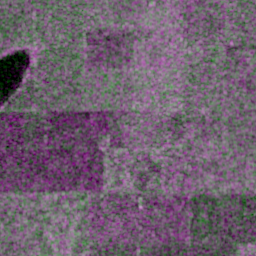
\includegraphics[width=0.155\textwidth]{img/ablation/sample_1/sar.png} &
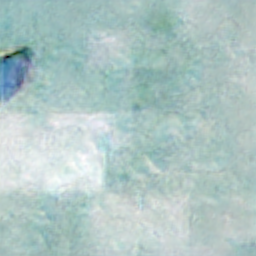
\includegraphics[width=0.155\textwidth]{img/ablation/sample_1/none.png} &
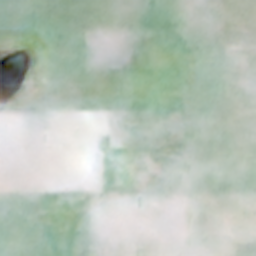
\includegraphics[width=0.155\textwidth]{img/ablation/sample_1/ssim.png} &
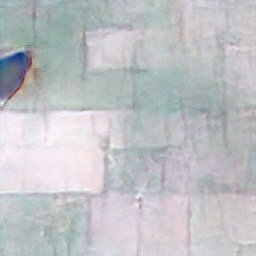
\includegraphics[width=0.155\textwidth]{img/ablation/sample_1/lpips.png} &
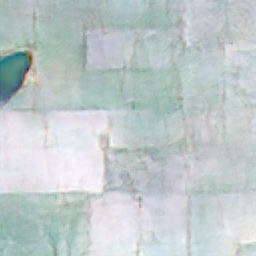
\includegraphics[width=0.155\textwidth]{img/ablation/sample_1/all.png} &
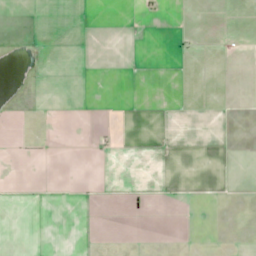
\includegraphics[width=0.155\textwidth]{img/ablation/sample_1/gt.png} \\
% ------------------- Row 2 -------------------
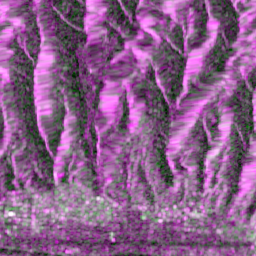
\includegraphics[width=0.155\textwidth]{img/ablation/sample_2/sar.png} &
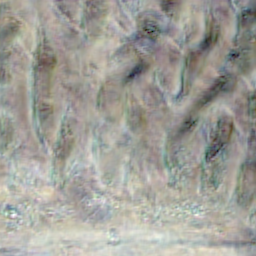
\includegraphics[width=0.155\textwidth]{img/ablation/sample_2/none.png} &
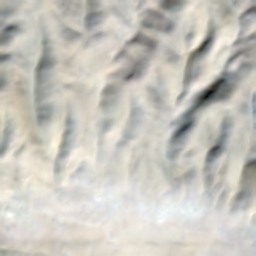
\includegraphics[width=0.155\textwidth]{img/ablation/sample_2/ssim.png} &
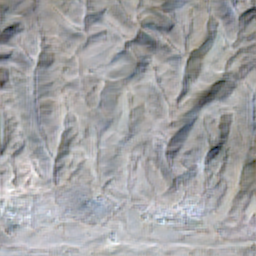
\includegraphics[width=0.155\textwidth]{img/ablation/sample_2/lpips.png} &
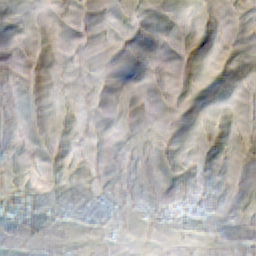
\includegraphics[width=0.155\textwidth]{img/ablation/sample_2/all.png} &
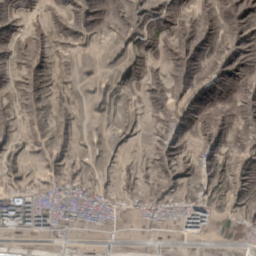
\includegraphics[width=0.155\textwidth]{img/ablation/sample_2/gt.png} \\
% ------------------- Row 3 -------------------
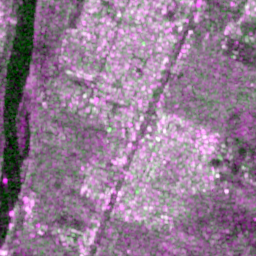
\includegraphics[width=0.155\textwidth]{img/ablation/sample_3/sar.png} &
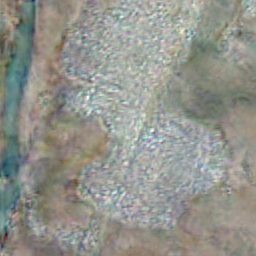
\includegraphics[width=0.155\textwidth]{img/ablation/sample_3/none.png} &
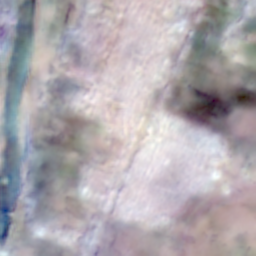
\includegraphics[width=0.155\textwidth]{img/ablation/sample_3/ssim.png} &
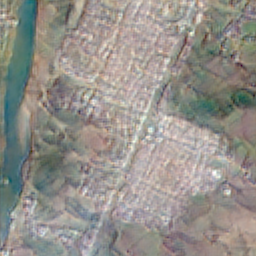
\includegraphics[width=0.155\textwidth]{img/ablation/sample_3/lpips.png} &
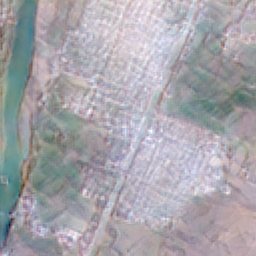
\includegraphics[width=0.155\textwidth]{img/ablation/sample_3/all.png} &
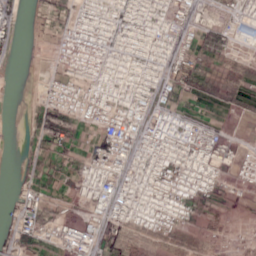
\includegraphics[width=0.155\textwidth]{img/ablation/sample_3/gt.png} \\
% ------------------- Row 4 -------------------
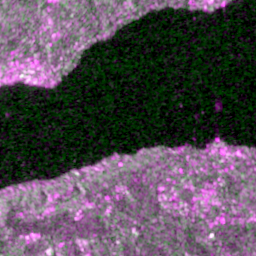
\includegraphics[width=0.155\textwidth]{img/ablation/sample_4/sar.png} &
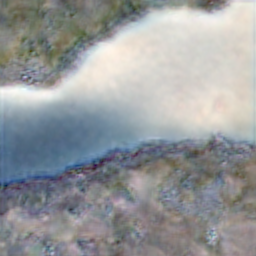
\includegraphics[width=0.155\textwidth]{img/ablation/sample_4/none.png} &
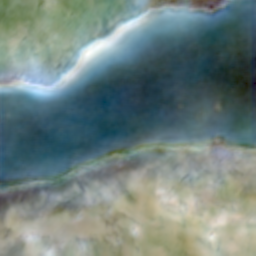
\includegraphics[width=0.155\textwidth]{img/ablation/sample_4/ssim.png} &
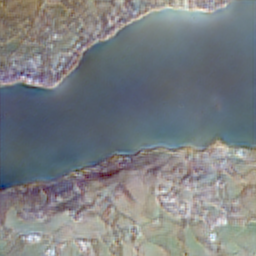
\includegraphics[width=0.155\textwidth]{img/ablation/sample_4/lpips.png} &
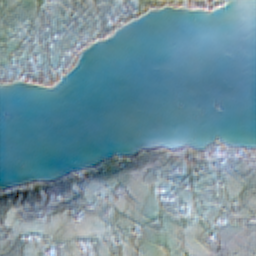
\includegraphics[width=0.155\textwidth]{img/ablation/sample_4/all.png} &
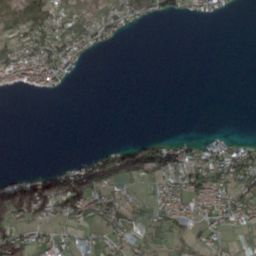
\includegraphics[width=0.155\textwidth]{img/ablation/sample_4/gt.png} \\
% \bottomrule
\end{tabular}

\caption{%
Qualitative ablation results showing representative samples (rows) under four configurations (columns):\\
\textbf{(a)}~Input SAR (VV+VH)\\
\textbf{(b)}~$\mathcal{L}_{\text{GAN}}{+}\mathcal{L}_{\text{L1}}$\\
\textbf{(c)}~$\mathcal{L}_{\text{GAN}}{+}\mathcal{L}_{\text{L1}}{+}\mathcal{L}_{\text{SSIM}}$\\
\textbf{(d)}~$\mathcal{L}_{\text{GAN}}{+}\mathcal{L}_{\text{L1}}{+}\mathcal{L}_{\text{LPIPS}}$\\
\textbf{(e)}~all four losses combined\\ 
\textbf{(f)}~ground-truth Sentinel-2 optical image.
}
\label{fig:ablation_samples}
\end{figure}

\subsubsection*{Discussion}
The results indicate that the combination of $\mathcal{L}_{\text{SSIM}}$ and $\mathcal{L}_{\text{LPIPS}}$ with the baseline adversarial and $\mathrm{L1}$ losses improves both perceptual quality and structural fidelity. 
Models trained with only $\mathcal{L}_{\text{GAN}}$ and $\mathcal{L}_{\text{L1}}$ tend to produce smoother images with limited high-frequency detail. 
Adding $\mathcal{L}_{\text{SSIM}}$ enhances edge sharpness and local contrast, while the inclusion of $\mathcal{L}_{\text{LPIPS}}$ yields more realistic color and texture distributions. 
The full combination of all four losses achieves the best balance between pixel-level accuracy, perceptual realism, and structural coherence.
